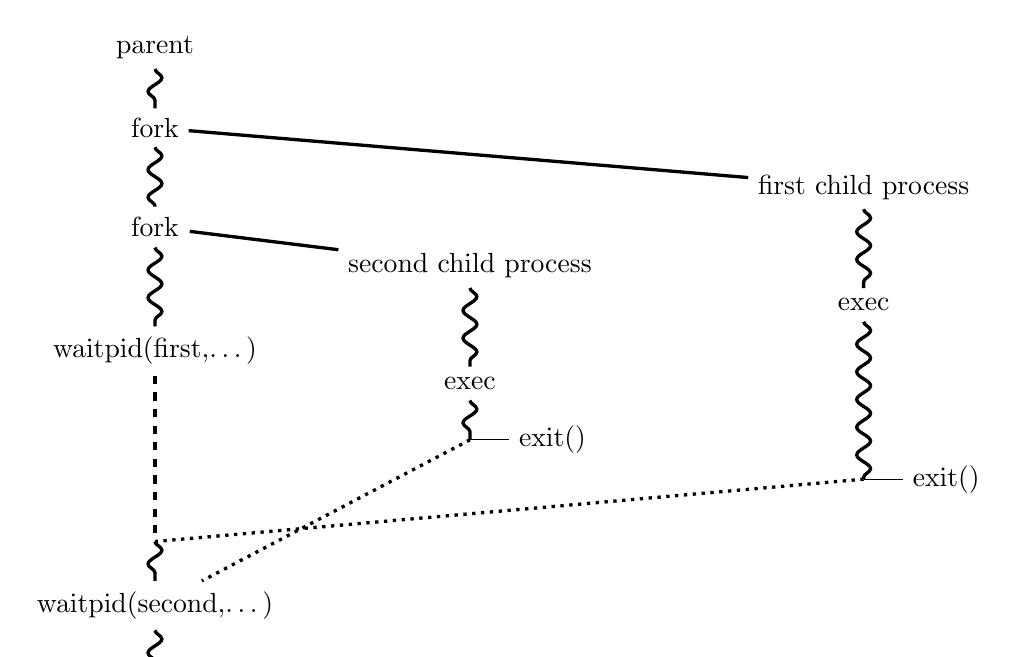
\begin{tikzpicture}
\tikzset{
    thread/.style={very thick,draw,decorate,decoration=snake},
    split/.style={very thick,draw},
    marker/.style={thin,draw},
}
\path[thread] (0, 0) --  (0, -.5);
\node[anchor=south] at (0,0) {parent};
\node[anchor=north] (fork mark 1) at (0, -.5) {fork};
\draw[thread] (fork mark 1) -- ++(0, -1) node[below] (fork mark 2) {fork};
\draw[thread] (fork mark 2.south) -- ++(0, -1) node[below] (wait 1 start) {waitpid(first,\ldots)};
\node (child 1 start) at (9, -1.5) {first child process};
\node (child 2 start) at (4, -2.5) {second child process};
\path[split] (fork mark 1) --  (child 1 start);
\path[split] (fork mark 2) --  (child 2 start);
\path[thread] (child 1 start.south) -- ++(0, -1) node[below] (exec 1) {exec};
\path[thread] (exec 1.south) -- ++(0, -2) coordinate (exec 1 done);
\path[marker] (exec 1 done) -- ++(.5, 0) node[right] {exit()};
\path[thread] (child 2 start.south) -- ++(0, -1) node[below] (exec 2) {exec};
\path[thread] (exec 2.south) -- ++ (0, -0.5) coordinate (exec 2 done);
\path[marker] (exec 2 done) -- ++(.5, 0) node[right] {exit()};
\path[split,dotted] (exec 1 done) -- (0, -6) coordinate (wait 1 done);;
\draw[very thick,dashed] (wait 1 start) -- (wait 1 done);
\draw[thread] (wait 1 done) -- ++(0, -.5) node[below] (wait 2 start) { waitpid(second,\ldots) };
\path[split,dotted] (exec 2 done) -- (wait 2 start);
\draw[overlay,thread] (wait 2 start.south) -- ++ (0, -2);
\end{tikzpicture}